\documentclass{article}
\usepackage{epsfig,graphicx,epsf,subfigure, amssymb, amsmath, float}
\usepackage{hyperref}
\usepackage[letterpaper, total={6.5in, 9in}]{geometry}
\author{Oscar Wang, David Zhou, Andrew Gauthier, David Zhang}
\date{\today}
\title{ECE 458 Evolution 2 Write Up}
\begin{document}
\maketitle
\section{Design Choices}
\subsection{Ruby on Rails}
As it turns out, Ruby on Rails has been both a blessing and a curse.  It has allowed us to quickly change our code to accomodate most of the new features, but it has also made some features particularly difficult to implement.  In particular, we have still not been able to implement an intuitive way of choosing the date range; we found a Ruby Gem specifically designed for this feature but have had problems integrating it into our program.  We also had problems with NetID authentication, as we will describe in a later section.  Overall, this seems to be the tradeoff we signed up for when we chose Ruby on Rails--its simplicity allowed us to quickly modify our code but also created limitations that we are still trying to surmount.\par
Another reason we chose Ruby on Rails was because of its familarity, but even this was not as great of a benefit as we initially thought.  While three of us have extensive experience with Ruby on Rails, one of us (David Zhou) has no experience with it at all.  One thing we should have done in the beginning was spend a few meetings explaining and teach him Ruby on Rails, because it would have increased our overall productivity later on.  We also should have given a little more consideration to other languages--especially Java, since this is a language that all of us have experience with.  If even one portion of the project was written in Java, it would ensure that all of us would be able to contribute to some part of the project at any time.
\subsection{PostgreSQL}
PostgreSQL is still a nightmare to work with on windows machines, but we got around this by setting up linux VMs through the Duke VM manager.  Once we set PostgreSQL up on the virtual machines (which involved some complicated troubleshooting involving users and permissions) it has not given us any trouble since.  The only limitations of our decision to use PostgreSQL are the limitations that come with any relational database.  So far, we have been able to work around them by carefully implementing our models.  If we decide that future implementations are significantly easier to implement with a non-relational database, we may consider switching, but for now we are happy with this decision.
\subsection{Heroku}
At the end of our last evolution, we were considering discarding Heroku entirely, but we have decided to stay on it for the time being.  We have not noticed a significant increase in speed on the VMs, and the VMs came with their own set of problems.  They seem to time out after about half an hour, which makes them unreliable for use as a production server.  Furthermore, Heroku handles client-server encryption automatically, while additional software needs to be installed on the VMs to add this feature.  We have contacted OIT about the time-out problem and are still waiting for a response.  Either way, we currently have bigger problems to tackle, and trying to get the VMs to work as production servers does not seem to offer significantly high return on investment.  Because we managed to resolve our earlier problems between Heroku and PostgreSQL, Heroku seems like the best choice moving foward.
\section{Program Organization}
\begin{figure}[h]
\centering
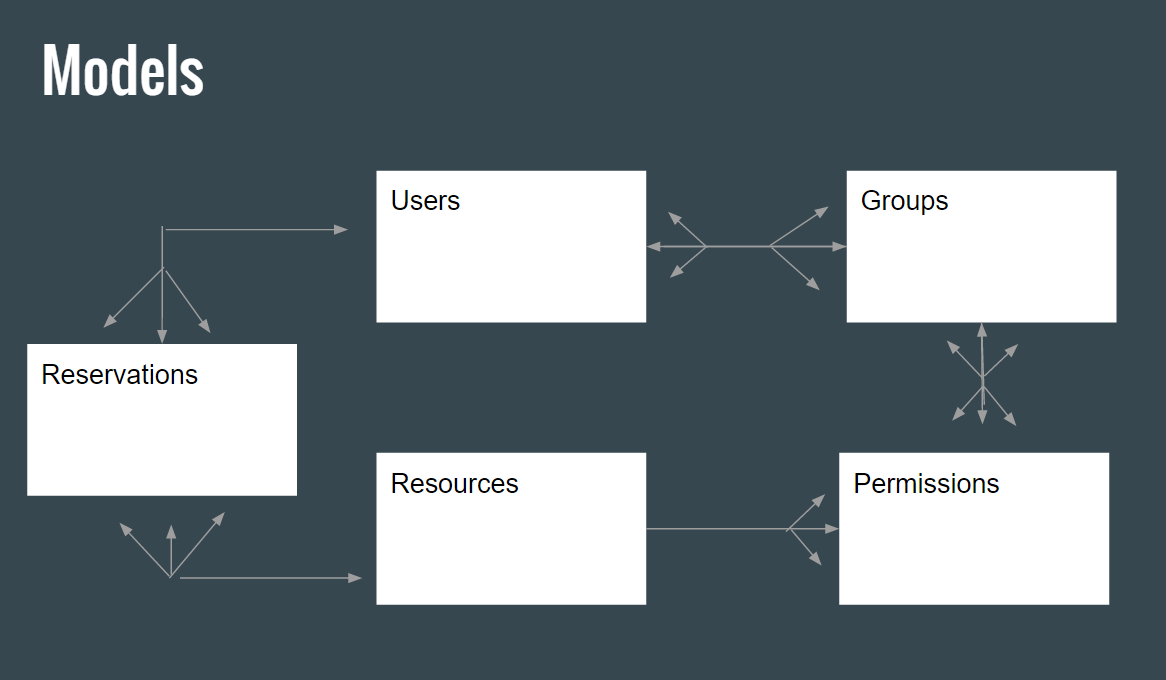
\includegraphics[width=5in]{snip}
\caption{Interactions Between the Design Models}
\end{figure}
\subsection{Models}
In order to add the management and permission access features, we had to add two new models: groups and permissions. The groups model has a has\_and\_belongs\_to\_many relationship with the users, so that a user can be in as many groups as possible, and each group can have as many users as possible. We made the decision to have users initialize in their own groups, in order to make it easy to treat users and groups as the same thing (like giving a certain user management rather than a group). The permissions model was a little tricky. Initially we thought of having the model almost as a join table, with a belongs\_to relationship for both the group and resource. However, we realized it would be easier to just have a resource and have another join table for groups, so we would only need two permissions per resource: a view access one and a reserve access one. We also had to make slight changes to our user model by incorporating the simple\_token\_auth gem, in order to help with the API authentication.

\subsection{Controllers}
We made several changes to the controllers. Most notably, we had to add the groups controller, in order to take into consideration adding groups. The controller itself is pretty simple and similar to the other controllers and rails implicit CRUD operations. however, we did have to incorporate simple forms (technically part of the view, but helped a lot with the controller) in order to make it easy for there to just be a check box for the adding users to groups. The permissions was done in a similar way to tags last evolution, by adding to the resources controller. We added a permissions method that allowed user to add to a resources permissions (currently two permission exist: one for view access and one for reserve access). We also had to add four api controllers for the api. These controllers are very similar to the original, but had to work in json rather than rendering html. Unfortunately, there is a lot of duplicated code as a result, but we were not too sure how to have different outputs even though they were really similar. 

\subsection{Views}
One of our biggest goals for this evolution was improving the front end of our application, since it was anything but user friendly for our first evolution.  Last time, we were considering incorporating React.js into the project, but ultimately decided against doing that for this evolution because there was too high of a startup cost.  David Zhou, the person who primarily worked on the front end of this project, was already struggling to learn Ruby on Rails.  Learning the nuances and idiosyncrasies of the React syntax and structure while trying to incorporate it into the Ruby on Rails framework was too much of a startup cost.  Instead, we turned to the Twitter Bootstrap, which allowed us to quickly integrate prebuilt themes and stylesheets into our project to build a decent looking user interface in a manageable amount of time.  We may still look at React.js in the future if we encounter anything we cannot accomplish with the Bootstrap alone, but for now, we are content with leaving it out.  In addition to the additional learning curve, using React.js will also introduce more dependencies into our project that we might be able to avoid.  There is also plenty of documentation and examples online for integrating Bootstrap into Ruby on Rails that will make extending the front end for future evolutions easier.\par
We also managed to fix some of the unintuitive aspects of our user interface from last evolution, such as being unable to deselect tags.
\subsection{NetID authentication}
Unfortunately, we were not able to incorporate NetID authentication using OAuth2.  We all had particularly busy schedules in the few days we had after we received approval from OIT.  Furthermore, we made the mistake of linking our registration to our Heroku URL, which would have required us to repeatedly deploy our program in order to test it.  We also did not know how to debug the program once it had been deployed on Heroku, which made it extremely difficult to implement this feature on time.  We are planning to obtain another permission to allow us to work on this feature on our VMs, but this will unfortunately have to wait until next evolution.
\section{Evaluation and Future Plans}
The application is definitely starting to look better.  We can actually claim to have a basic front end this time, and we have created an application that satisfies most of the requirements.  It is definitely something that we are happier to present this time around.\par
However, there are several significant problems in our design that we are going to have to address before we even start thinking about the Evolution 3 requirements.  In particular:
\begin{itemize}
\item{One feature from the first evolution has still not been implemented: allowing the user to set a time-range for reservations.  This is something that needs to be fixed as soon as possible, and now that we have more experience with web UI, we have no more excuses for leaving this one out.}
\item{NetID authentication has not been integrated yet, as mentioned earlier.}
\item{There are a few bugs, or unintuitive nuances of our program that should be corrected.  For example, deleting the last resource of a particular tag does not get rid of the tag itself, and the tag just lingers in the database forever.}
\end{itemize}
For the next evolution, we need to get serious about fixing these problems, so that they do not still plague us when evolution 4 comes out.  We plan to start looking into this before spring break by acting on the following initiatives:
\begin{itemize}
\item{Hold a meeting or two just to get everyone up to date.  In addition to problems associated with inexperience with Ruby on Rails, we also need to make sure everyone has a sufficient understanding of the overall program.}
\item{Start aggressively debugging and polishing the project, so that everything from Evolutions 1 and 2 will be completely left behind before spring break.  This will allow us to approach Evolution 3 without any excess baggage from the first evolutions.}
\item{Meet consistently throughout the rest of our alloted time on this Evolution instead of leaving a majority of the work for last two weeks. We want to have a product we can be proud of when we are given our final Evolution of the semester.}
\end{itemize}
\section{Contributions}
\begin{itemize}
\item{Oscar Wang: Implemented extensions to the backend, worked on API, prepared the presentation}
\item{David Zhou: Worked on the front end, debugged, wrote and formatted the write-up}
\item{Andrew Gauthier: Implemented extensions to the backend, worked on API}
\item{David Zhang: Planning stuff}
\end{itemize}
\section{Appendix}

\begin{figure}[h]
\centering
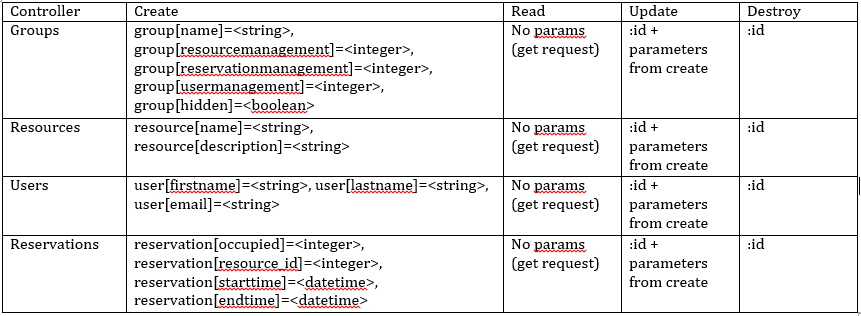
\includegraphics[width=6in]{table}
\caption{Table 1: API}
\end{figure}

\end{document}

